%Standard Header
\documentclass[11pt,a4paper,toc=listof,toc=bibliography]{scrartcl}
\usepackage[utf8]{inputenc}
\usepackage[ngerman]{babel}
\usepackage[T1]{fontenc}
\usepackage{amsmath}
\usepackage{amsfonts}
\usepackage{amssymb}
\usepackage[pdftex]{graphicx}

%\usepackage{epstopdf}                            %import .eps (from MATLAB)
\usepackage{geometry}
\usepackage{multirow}
\usepackage{pdfpages}                            %import pdf
\usepackage{textcomp}                            %degree celsius etc
\usepackage{gensymb}
\usepackage[hidelinks]{hyperref}                 %hidelinks removes red boxes from pdf
\usepackage[style=german, german=quotes]{csquotes}
\usepackage[backend=biber, style=numeric, citestyle=numeric, sorting=none]{biblatex}
\usepackage{float}

\usepackage[all,defaultlines=2]{nowidow}		%prevent Witwen and Schusterjungen
\usepackage{microtype}

\usepackage{color}
\usepackage{listings}                            %einbinden von Sourcecode

%\usepackage{chemfig}
\usepackage{upgreek}
\usepackage{chemmacros}
\usepackage{chemformula}

\addbibresource{../DATA/bibresource.bib}        %Standardpfad für .bib Datei des Projektes

\usepackage{lmodern}

%\KOMAoption{DIV}{12}

%%%% alte Definition:
%% \DeclareMathSymbol{,}{\mathpunct}{letters}{"3B}
%%%% neue Definition:
%%\DeclareMathSymbol{,}{\mathord}{letters}{"3B}       %removes space in mathmode
\DeclareMathSymbol{*}{\mathbin}{symbols}{"01}

\newcommand{\mlab}{MATLAB}
%\renewcommand{\figurename}{Abb.}    %for article/report and non KOMA-Classes
\renewcaptionname{ngerman}{\figurename}{Abb.}

\setlength{\parindent}{0pt}          %keine Einschübe bei neuem Absatz

\addtokomafont{disposition}{\rmfamily} % serifes in headings

%SI-Units and correct spacing according to ISO-31
\usepackage[range-phrase = \ldots~]{siunitx}
\sisetup{locale=DE}
\sisetup{inter-unit-product=\ensuremath{{}*{}}}
\sisetup{per-mode=symbol}
%Listings environment for sourcecode
%\renewcommand{\lstlistlistingname}{Sourcecode}     %name in listof"sourcecode"
%\renewcommand{\lstlistingname}{Code}            %captionPreName

\lstset{breaklines}
\lstset{numbers=left}
\lstset{frame=single}
%\lstset{language=Matlab}
\lstset{showstringspaces=false}
\lstset{ %
	backgroundcolor=\color{white},   % choose the background color
	basicstyle=\footnotesize,        % size of fonts used for the code
	breaklines=true,                 % automatic line breaking only at whitespace
	captionpos=b,                    % sets the caption-position to bottom
	commentstyle=\color{olive},      % comment style
	escapeinside={\%*}{*)},          % if you want to add LaTeX within your code
	keywordstyle=\color{blue},       % keyword style
	stringstyle=\color{magenta},     % string literal style
	extendedchars=true,
	literate={ä}{{\''a}}1 {ö}{{\''o}}1 {ü}{{\''u}}1 {ß}{{\ss}}1,
	inputencoding=utf8,
}

% Site-Header with KOMA
%\usepackage[headsepline]{scrlayer-scrpage}    %headsepline makes line under header
%\ihead{}        %Inner-Head
%\ohead{}                    %Outer-Head
%\pagestyle{scrheadings}                        %activate Headings
%\setkomafont{pageheadfoot}{\normalsize}        %normal fontsize for headline

\renewcommand{\mkbegdispquote}[2]{\glqq}
\renewcommand{\mkenddispquote}[2]{\grqq#2}
\renewcommand{\mkcitation}[1]{ \textsuperscript{[}#1\textsuperscript{]}}  

\hyphenation{}
\hyphenation{}

\begin{document}
\begin{titlepage}
	
	\begin{figure}[H]
		\begin{minipage}{0.5\textwidth}
			\centering
			
\includegraphics[width=0.8\textwidth]{../DATA/Logo_Uni-Kassel.pdf}
			%\caption{Kugel mit Stativ}
			%\label{fig3}
		\end{minipage}\hfill
		\begin{minipage}{0.5\textwidth}
			\centering
			
\includegraphics[width=0.8\textwidth]{../DATA/Logo_solar.png}
			%\caption{Druckmessbohrung Kugel}
			%\label{fig4}
		\end{minipage}
	\end{figure}
	
		\vspace{3cm}
	
	\centering
	{\scshape\LARGE Praktikum thermische Messtechnik\par}   %Title
	\vspace{1cm}
	{\scshape\Large Teil 3: Meteorologische Messgrößen \par}
	\vspace{1.5cm}
%	{\huge\bfseries  Neuartige Brennstoffzellenkonzepte: Hyform-PEMFC mit Ameisensäure, Bioprozesse auf Güllebasis - was geht noch?\par}  %Hauptüberschrift
	\vspace{2cm}
	{\Large Lena Völlinger \& Marvin Grosch\par}
	\vfill
	
	% Bottom of the page
	\begin{large}
		\begin{tabular}{l l}
			
			Praktikumstag: & 08.09.2020 \\
			Erstabgabe: & 05.10.2020\\
			Betreuer: & Markus Rusack \& Christoph Schmelzer\\
			Studiengang: & Master $\text{re}^2$\\
			Semester: & SoSe 2020\\
			Matrikelnr.: & 35597894, 35598242\\ 
		\end{tabular}
	\end{large}

\end{titlepage}

\pagenumbering{Roman}

\newpage
\tableofcontents
\listoffigures
\newpage

\pagenumbering{arabic}

\section{Einleitung}

Für den Versuch Temperaturmessung sollten verschiedene Temperatursensoren (Pt100 2L, Pt1000 2L, KTY 2L, NTC 2L) und ein Thermoelement Typ K an einem Metallblockkalibrator mit einem Pt-100 4L Referenzfühler, der zuvor an einer Wassertripelpunktzelle kalibriert wurde,  gemessen und deren Genauigkeit beurteilt werden. 
Die verschiedenen Temperaturensensoren wurden anhand von Fixpunkt- und Vergleichsmethode charakterisiert. 

Anschließend wurden Widerstandssensoren unterschiedlichen Typs mit einem Mulitmeter untersucht und Anhand ihrer Kennliniendiagramme identifiziert. 

Im dritten Teil wurde sich mit der berührungslosen Temperaturmessung befasst. Es erfolgte die Untersuchung verschiedener Materialien in einem temperierten Wasserbad mithilfe einer Wärmebildkamera. Dabei wurden die Unterschiede der Materialien und ihren Einfluss auf die Messung untersucht und analysiert. 
%\newpage
\section{Versuchsauswertung}

\subsection{Speicher A}

\subsubsection{UA-Wert Plattenwärmeübertrager}
Zur Bestimmung des UA-Wertes wurden die zu Beginn der Speicherbeladung aufgenommenen Messdaten verwendet. Diese sind in Abbildung \ref{fig:extWT} gezeigt. Für die Berechnung wurde der Stationäre Temperaturverlauf zwischen den Scans 150 und 270 gemittelt. Zusätzlich wurde der Volumenstrom des orangenen MIDs zum gegeben Zeitraum erfasst. 

\begin{figure}[H]
	\centering
	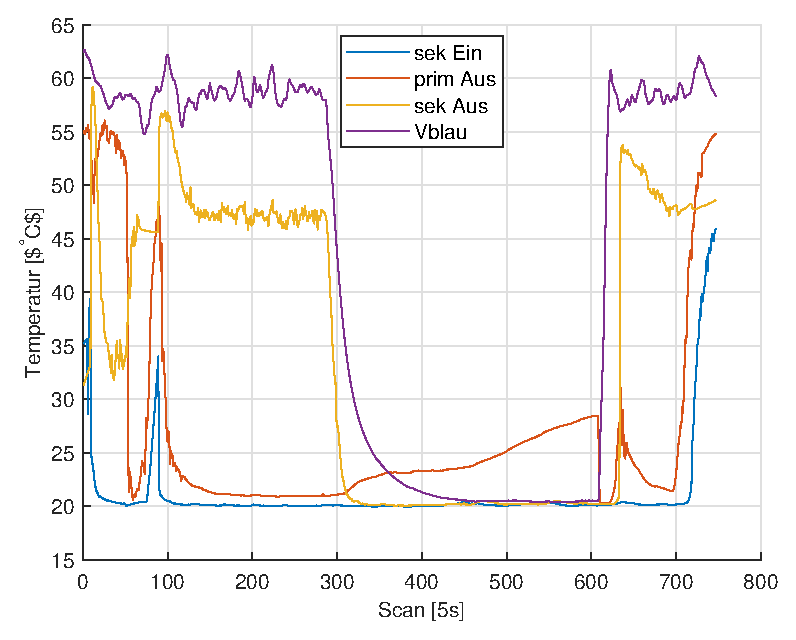
\includegraphics[width=0.7\textwidth]{../DATA/PlattenWT_A.eps}
	\caption[Temperaturverläufe des Platten-WÜT]{Temperaturverläufe des Platten-WÜT}
	\label{fig:extWT}
\end{figure}

Die benötigten Temperaturen sind in folgender Tabelle zusammengefasst. Der Volumenstrom beträgt 0,0874 $\pm1,8614*10^{-4} \frac{m^3}{h}$.

\begin{table}[H]
	\centering
	
	\begin{tabular}{l|c}
		
		
		\textbf{Messwert} & \textbf{Mittelwert} [T] in ${\celsius}$\\
		\hline
	$T_{sek,ein}$ & 20,06 $\pm$0,04\\
	$T_{sek,aus}$ & 47,16 $\pm$0,57\\
	$T_{prim,ein}$ & 58,85 $\pm$0,84\\
	$T_{prim,aus}$ & 21,02 $\pm$0,10\\

	%$T_{sek,ein}$ & 20,0646 $\pm$0,0397\\
	%$T_{sek,aus}$ & 47,1604 $\pm$0,5687\\
	%$T_{prim,ein}$ & 58,8494 $\pm$0,8431\\
	%$T_{prim,aus}$ & 21,0185 $\pm$0,0965\\	
	\end{tabular}
\caption[UA-Wert-Bestimmung Speicher A]{UA-Wert-Bestimmung Speicher A}
\label{tab:extWT}
\end{table}
Die Berechnung erfolgt gemäß Gleichung \ref{eq:QextWT} bis \ref{eq:UAext}. Näherungsweise wurden eine Wasserdichte von \SI{1000}{\kilogram\per\cubic\meter} und eine Wärmekapazität von \SI{4190}{\joule\per\kilogram\kelvin} angenommen.
\begin{equation}
	\label{eq:QextWT}
	\dot Q_{WÜT} = \rho_{w} * \dot V_{MID,orange} * c_{p,w} * (T_{prim,ein}-T_{prim,aus}) = \SI{3850}{\watt}
\end{equation}

\begin{center}
	\begin{small}
	$\dot Q_{WÜT}$:Wärmestrom am WÜT,	
	$\rho_{w}$:	Dichte von Wasser,
	$c_{p,w}$: Wärmekapazität von Wasser
	\end{small}
\end{center}

\begin{equation}
	\label{eq:DeltaTm}
%	\Delta T_{m} = \frac{|\Delta T_{0} - \Delta T_{1}|}{ln(\frac{\Delta T_{0}}{\Delta T_{1}})} = \SI{4,28}{\kelvin}
	\Delta T_{m} = \frac{|\Delta T_{0} - \Delta T_{1}|}{ln(\frac{\Delta T_{0}}{\Delta T_{1}})} = \SI{4,2840}{\kelvin}
\end{equation}
\begin{center}
	\begin{small}
		$\Delta T_{m}$: Mittlere Temperaturdifferenz
	\end{small}
\end{center}

mit
\begin{equation}
	\label{eq:DeltaT0}
	\Delta T_{0} = T_{prim,ein} - T_{sek,aus}
\end{equation}

\begin{equation}
	\label{eq:DeltaT1}
	\Delta T_{1} = T_{prim,aus} - T_{sek,ein}
\end{equation}
Der UA Wert ergibt sich aus dem Quotienten von Gleichung \ref{eq:QextWT} und \ref{eq:DeltaTm}.
\begin{equation}
	\label{eq:UAext}
	UA_{WÜT} = \frac{\dot Q_{WÜT}}{\Delta T_{m}} = \SI{898,7}{\watt\per\kelvin}
\end{equation}

\subsubsection{Füllvorgang}
Bei der Befüllung wurde der Temperaturverlauf an der Messlanze beobachtet und aufgezeichnet. Abbildung \ref{fig:SpAfill} zeigt den zugehörigen Datensatz mit den verschiedenen Messpunkten.

\begin{figure}[H]
	\centering
	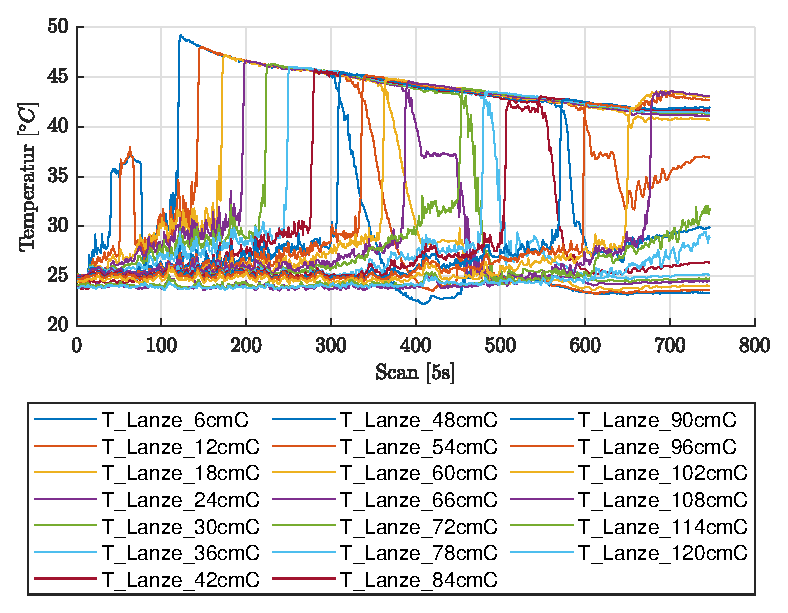
\includegraphics[width=0.9\textwidth]{../DATA/SpA_Lanzen.eps}
	\caption[Temperaturverlauf Speicher A]{Temperaturverlauf der Befüllung von Speicher A}
	\label{fig:SpAfill}
\end{figure}

Zunächst wurde erhitztes Wasser bis zur \SI{30}{\liter} Markierung des Speichers durch den Bodeneinlass aufgefüllt. Beim eintauchen in das Wasser steigt die gemessene Temperatur an der jeweiligen Lanzenhöhe sehr schnell an. Aufgrund der Wärmeverluste und der Wärmeverteilung durch die Temperaturschichtung kann die Speichereintrittstemperatur nicht überall gehalten werden, an den höheren Sensoren wird daher eine etwas niedrigere Temperatur gemessen. Im nächsten Schritt wird der Speicher über die Prallplatte mit kaltem Wasser bis zur \SI{50}{\liter} Markierung gefüllt. (Scan 300 bis 450). Die Temperatur fällt an den unteren Sensoren ab, an den oberen Sensoren bleibt die Temperatur stabil oder sinkt nur leicht. Beim wechsel auf den Bodeneinlass (Scan 450 bis 500) wird die Schicht bis zu einer Speicherhöhe von \SI{36}{\centi\meter} gestört. Beim Wechsel auf das Steigrohr (Scan 500 bis 650) tritt zunächst kein Temperatursprung auf, bis schließlich die Temperaturen auf einer Höhe zwischen 40 und \SI{50}{\centi\meter}abfallen. Ein Zeichen dafür, dass die Schichtung funktioniert und durch den Zufluss des kalten Wassers die warme Schicht angehoben wird. Beim abschließenden Wechsel auf heißes Wasser ist ein Temperaturhub an den obersten Schichten festzustellen. Auch in diesem Fall erfüllt das Steigrohr seinen Zweck.

\subsection{Speicher B}
\subsubsection{UA-Wert Rohrbündel}
Bei der Ermittlung des UA-Wertes wird analog zum vorherigen Versuchsteil vorgegangen. Da das Steigrohr fast den  Boden des Speichers berührt, wird dieses als Sekundärseite des Wärmeübertragers betrachtet. Der unterste Messpunkt der Temperaturlanze dient als Einlass, der am oberen Ende des Steigrohres montierte Temperaturfühler als Auslass. Abbildung \ref{fig:intWT} zeigt den Messverlauf der beschriebenen Größen. Zur Berechnung wurden die letzten 15 Scans gemittelt und in Tabelle \ref{tab:intWT} zusammengefasst. Der blaue MID erfasst den Volumenstrom im Steigrohr, welcher nach Abzug des gegebenen Messfehlers \SI{0,1175}{\cubic\meter\per\hour} beträgt.

\begin{figure}[H]
	\centering
	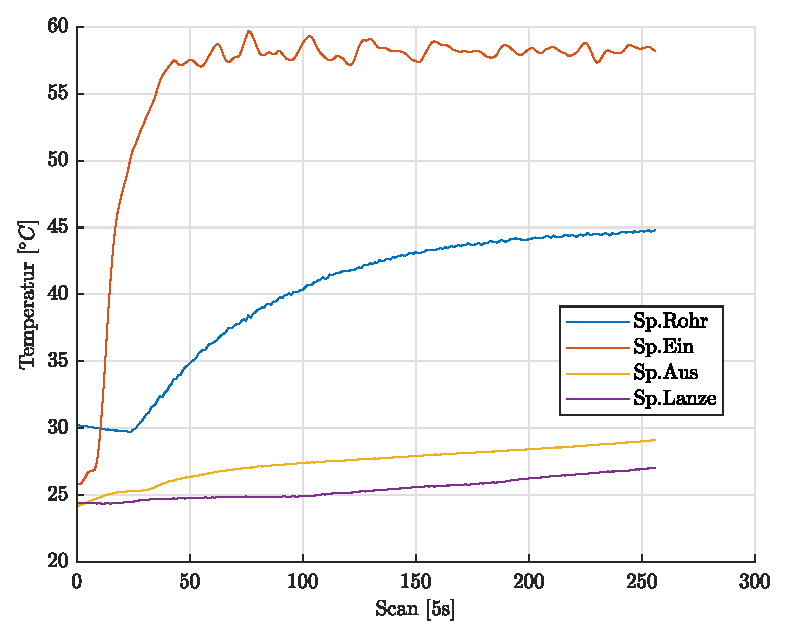
\includegraphics[width=0.8\textwidth]{../DATA/RohrWT_B.eps}
	\caption[Temperaturverläufe des Rohr-WÜT]{Temperaturverläufe des Rohr-WÜT}
	\label{fig:intWT}
\end{figure}


\begin{table}[H]
	\centering
	
	\begin{tabular}{l|c}
		
		
		\textbf{Messwert} & \textbf{Mittelwert} [T] in ${\celsius}$\\
		\hline
		$T_{Lanze,6cm}$ & 26,63 $\pm$0,23\\
		$T_{pipe}$ & 44,47 $\pm$0,18\\
		$T_{WT,ein}$ & 58,22 $\pm$0,31\\
		$T_{WT,aus}$ & 28,74 $\pm$0,20\\
	
%		$T_{sek,ein}$ & 26,6349 $\pm$0,2263\\
%		$T_{sek,aus}$ & 44,4749 $\pm$0,1786\\
%		$T_{prim,ein}$ & 58,2179 $\pm$0,3096\\
%		$T_{prim,aus}$ & 28,7390 $\pm$0,1990\\
		
	\end{tabular}
\caption[UA-Wert-Bestimmung Speicher B]{UA-Wert-Bestimmung Speicher B}
\label{tab:intWT}
\end{table}

Die Berechnung nach Gleichung \ref{eq:UAext} ergibt einen UA-Wert von

\begin{equation}
	\label{eq:UAint}
%	UA_{WÜT} = \frac{\SI{4032,8}{\watt}}{\SI{6.2019}{\kelvin}} = \SI{650,3}{\watt\per\kelvin}
		UA_{WÜT} = \frac{\SI{4032,8}{\watt}}{\SI{6,20}{\kelvin}} = \SI{650,3}{\watt\per\kelvin}
\end{equation}

\subsubsection{Volumenstrom Steigrohr}
Neben der Messung mittels MID kann der Volumenstrom im Steigrohr auch über die sekundärseitige Energiebilanz des Wärmeübertragers bestimmt werden. Umstellen von Gleichung \ref{eq:QextWT} und Einsetzen der Temperaturen und des Wärmestroms aus Gleichung \ref{eq:UAint} ergibt

\begin{equation}
	\label{eq:Vdot}
	\dot V_{Rohr}  =\frac{\dot Q_{WÜT}}{\rho_{w} *  * c_{p,w} * (T_{sek,aus}-T_{sek,ein})}  = \SI{0,194}{\cubic\meter\per\hour}
\end{equation}

Der berechnete Wert liegt 65\% über dem ausgegebenen Wert des MID. Grund dafür könnte das stark vereinfachte Modell zur Beschreibung des Wärmeübertragers sein. Die Temperatur der Sekundärseite wurde lediglich anhand der Messlanze geschätzt und komplexere Strömungseffekte im und am Steigrohr wurden vernachlässigt. Weiterhin wurde der Volumenstrom über die Dichteintegrale bestimmt (Gl. \ref{eq:int}).
\begin{multline}
	\label{eq:int}
	\Delta p_{drive}=g*\biggl|\int_{h_{1}}^{h_{2}}\rho(T_{WS1})\,dh'-\int_{h_{1}}^{h_{2}}\rho(T_{WS2})\,dh'\biggl|=g*\biggl|(\rho(T_{Lanze,6cm})*h_{Boden}\\+\rho((T_{WÜT,ein}+T_{WÜT,aus})/2)*h_{WÜT}+\rho(T_{pipe})*h_{pipe})-\sum\limits_{i=1}^{18}(\rho(T_{i})*\Delta h_{i})\biggl|
\end{multline}
Folgende Werte wurden neben den Temperaturen aus Tab. \ref{tab:intWT} verwendet:

\begin{table}[H]
	\centering
	
	\begin{tabular}{l|c}
		
		
		\textbf{Parameter} & \textbf{Wert}\\
		\hline
		g & \SI{9,81}{\meter\per\square\second}\\
		$h_{Boden}$ & \SI{0,12}{\meter}   \\
		$h_{WÜT}$ & \SI{0,23}{\meter}   \\
		$h_{pipe}$ & \SI{0,73}{\meter}   \\
		$\Delta h_{i}$ & \SI{0,06}{\meter}   \\
	\end{tabular}
\caption[Parameter zu Bestimmung der thermosiphonischen Strömung.]{Parameter zu Bestimmung der thermosiphonischen Strömung.}
\label{tab:par}
\end{table}
Zur Bestimmung der temperaturabhängigen Dichte von Wasser wurde folgende Näherung verwendet und in Gl. \ref{eq:int} implementiert:

\begin{equation}
	\label{eq:dens}
	\rho(T)=\frac{\SI{1000}{\kilogram\per\cubic\meter}}{1+0.0002*T}
\end{equation}
Der Antriebsdruck ergibt sich zu \SI{74,35}{\pascal}. Weiterhin gilt:
\begin{align}
	\Delta p_{drive}-\zeta*\frac{\rho(T_{pipe})}{2}*v_{pipe}^2=0\\
	\zeta=1,44+\frac{0,3164}{Re^{0,25}}*\frac{h_{pipe}}{d_{pipe}}\\
	Re=\frac{\rho(T_{pipe})*v_{pipe}*d_{pipe}}{\eta}
\end{align}
Einsetzen von Gl. 12 in Gl. 11 in Gl. 10 und Berechnung der Nullstelle ($v_{pipe}$) ergibt bei einem Steigrohrdurchmesser von \SI{16}{mm} einen Volumenstrom von \SI{0,155}{\cubic\meter\per\hour}. Dieser Wert liegt mit einer Abweichung von 32\,\% näher an der Anzeige des MID. Abblidung \ref{fig:temp} zeigt, dass im verwendeten Datensatz keine ordentliche Temperaturschichtung im Speicher vorlag. Dieser Aspekt kann die thermosiphonische Berechnung verfälschen. Während bereits in der Speichermitte erhöhte Temperaturen auftreten, ist eine Temperaturspreizung am oberen Ende des Steigrohrs verglichen mit der Messlanze zu beobachten. 
\begin{figure}[H]
	\centering
	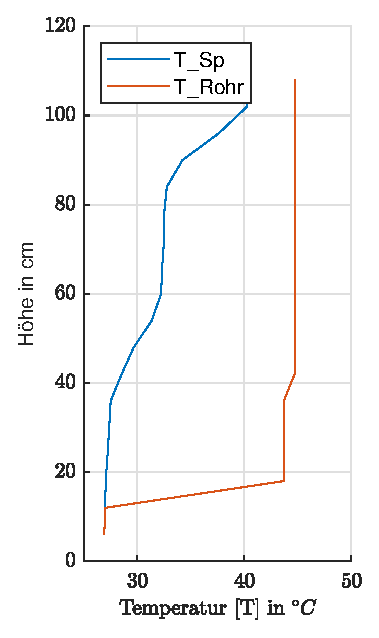
\includegraphics[width=0.32\textwidth]{../DATA/siphon.eps}
	\caption[Temperaturschichtung Speicher B]{Temperaturschichtung Speicher B}
	\label{fig:temp}
\end{figure}
Die thermosiphonische Strömung kommt zum Erliegen, wenn sich die Temperatur (und somit die Dichte) innerhalb und außerhalb des Steigrohres angleicht. In diesem Fall gilt für die antreibende Druckdifferenz $\Delta p_{drive}=0$.  



%\input{sections/03_Neuartige_Brennstoffzellenkonzepte}
%\newpage
%\input{sections/04_Zusammenfassung_und_Ausblick}

\newpage
%\printbibliography


\end{document}